%%%%%%%%%%%%%%%%%%%%%%%%%%%%%%%%%%%%%%%%%%%%%%%%%%%%%%%%%%%%%%%%%%%%%%%%%%%%%%%%
\chapter{Реализация алгоритма}
\label{chap:impl}
%%%%%%%%%%%%%%%%%%%%%%%%%%%%%%%%%%%%%%%%%%%%%%%%%%%%%%%%%%%%%%%%%%%%%%%%%%%%%%%%

Для оценивания эффективности предложенного в разделе~\ref{chap:dev} решения, реализауем его в виде программной библиотеки (реализация алгоритма). Результаты, полученные с помощью данной реализации будут использованы в разделе~\ref{chap:quality} для проведения экспертного анализа.

В данном разделе рассматриваются некоторые аспекты реализации описанного алгоритма извлечения ВОП из обращений в службу поддержки, описана структура проекта, определены используемые технологии. Полный текст программы  реализации алгоритма доступен на прилагаемом к данной работе CD-диске.

%%%%%%%%%%%%%%%%%%%%%%%%%%%%%%%%%%%%%%%%%%%%%%%%%%%%%%%%%%%%%%%%%%%%%%%%%%%%%%%%
\section{Используемые технологии}
%%%%%%%%%%%%%%%%%%%%%%%%%%%%%%%%%%%%%%%%%%%%%%%%%%%%%%%%%%%%%%%%%%%%%%%%%%%%%%%%
Для реализации алгоритма использовались следующие технологии: Java, Kotlin, Gradle, Git, JUnit, MongoDB, Mallet.

В качестве языка программирования используется \textit{Kotlin}. Kotlin~--- это активно развивающийся язык программирования общего назначения для JVM, к достоинствам которого относятся:

\nomenclature{JVM}{Java Virtual Machine}

\begin{itemize*}
\item Вывод типов;
\item Статическая типизация;
\item Мультипарадигменность;
\item Nullable типы данных;
\item Выразительный синтаксис;
\item Совместимость с java кодом.
\end{itemize*}

Описанные выше достоинста языка позволяют решать поставленные перед программистом задачи более эффективно, чем при использовании java. При этом, благодаря совместимости с java, сохраняется возможность исползования большого количества существующих java-библиотек.

На момент написания данной работы, Kotlin поддерживает Gradle, Maven и Ant для автоматической сборки проектов. \textit{Gradle}~--- система автоматической сборки, предоставляющая DSL на языке Groovy, и, по сравнению с другими решениями, использующими XML, позволяет писать более компактные сценарии сборки.

\nomenclature{DSL}{Domain-Specific Language, Предметно-ориентированный язык}
\nomenclature{XML}{eXtensible Markup Language}
\nomenclature{JSON}{JavaScript Object Notation}
\nomenclature{СУБД}{Система Управления Базами Данных}

\textit{Git}~--- система контроля версий, используемая командой YouTrack.

\textit{JUnit}~--- библиотека для модульного тестирования программного обеспечения. Совместима с Kotlin.

Для хранения данных используется \textit{MongoDB}. Для работы с обращениями в службу поддержки команда YouTrack использует Zendesk. Загружаемые из Zendesk данные имеют JSON формат. Поскольку MongoDB использует JSON-подобные документы и схему базы данных, было решено использовать данную СУБД, вместо реляционных баз данных.

\textit{Mallet}~\cite{MALLET}~--- библиотека на java, которая содержит реализацию необходимой тематической модели (LDA). Данная реализация написана в 2009 году, является наиболее 'взрослой' и развитой реализацией LDA. Подробнее о выборе реализации LDA написано в секции~\ref{sec:lda_choose}.

%%%%%%%%%%%%%%%%%%%%%%%%%%%%%%%%%%%%%%%%%%%%%%%%%%%%%%%%%%%%%%%%%%%%%%%%%%%%%%%%
\section{Структура проекта}
%%%%%%%%%%%%%%%%%%%%%%%%%%%%%%%%%%%%%%%%%%%%%%%%%%%%%%%%%%%%%%%%%%%%%%%%%%%%%%%%

Структура проекта представляет собой набор пакетов (\textit{packages}), каждый из которых соответсвует одному из этапов извлечения ВОП, описанными в разделе~\ref{chap:dev}. Общая структура пакетов предствалена на рисунке~\ref{fig:pckgs}. 

\begin{figure}[tph!]
\centerline{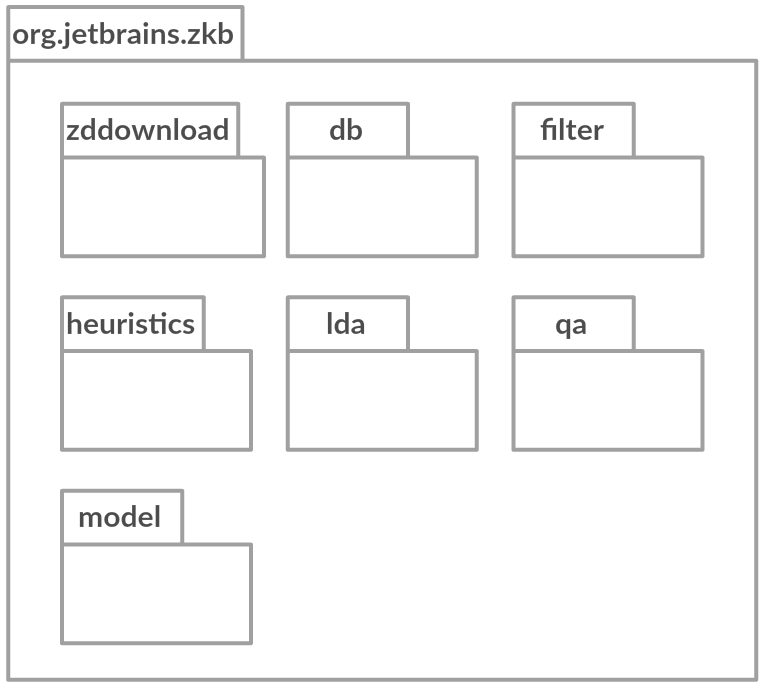
\includegraphics[width=7.5cm]{fig/pckgs.png}}
    \caption{Обобщенная структура пакетов реализации алгоритма}
    \label{fig:pckgs}
\end{figure}

Каждый из пакетов выполняет соответсвующую ему задачу:

\begin{itemize*}
\item org.jetbrains.zkb.zddownload~--- загрузка данных из Zendesk и сохранение их в базу данных;
\item org.jetbrains.zkb.model~--- модель данных, классы Comment (комментарий), QAPair (пара вопрос-ответ) и так далее.
\item org.jetbrains.zkb.db~--- данный пакет содержит классы отвечающие за зваимодействие с базой данных;
\item org.jetbrains.zkb.filter~--- содержит фильтры различного рода для анализируемых данных;
\item org.jetbrains.zkb.heuristics~--- эвристики предобработки;
\item org.jetbrains.zkb.lda~--- построение тематичечской модели анализируемых данных;
\item org.jetbrains.zkb.qa~--- формирование ВОП;

\end{itemize*}

Далее каждый из пакетов рассматривается более подробно.

%%%%%%%%%%%%%%%%%%%%%%%%%%%%%%%%%%%%%%%%%%%%%%%%%%%%%%%%%%%%%%%%%%%%%%%%%%%%%%%%
\section{Получение исходных данных}
\label{sec:zddwn}
%%%%%%%%%%%%%%%%%%%%%%%%%%%%%%%%%%%%%%%%%%%%%%%%%%%%%%%%%%%%%%%%%%%%%%%%%%%%%%%%

Пакет \textbf{org.jetbrains.zkb.zddownload} содержит программный код отвечающий за загрузку данных из Zendesk.

Взаимодействие с Zendesk происходит через REST API~\cite{zdapi}. В Zendesk обращение представлено такой сущностью, как \quotes{Ticket} (тикет). Тикет содержит ряд метаинформации об обращении: уникальный идентификатор обращения, дата и время создания, дата и время последнего обновления, статус обращения, уникальный идентификатор инициатора и так далее~--- при этом информация о соответсвующих данному обращению комментариях отсутсвует.

\nomenclature{REST}{Representational State Transfer}
\nomenclature{API}{Application Programming Interface, программный интерфейс приложения}

Комментарии представлены сущностью \quotes{Comment}, содержащей текст комментария и также некоторую дополнительную метаинформацию: уникальные идентификаторы комментария и автора, дата и время создания и так далее. Таким боразом, для получения достаточной для дальней обработки информации об обном обращении, необходимо загрузить:

\begin{enumerate*}
\item Объект представляющий обращений (Ticket);
\item Все комментарии (Comment), пренадлежащие данному обращению;
\end{enumerate*}

Для загрузки данных использовался клиент\footnote{https://github.com/cloudbees/zendesk-java-client \label{fn:zdcl}} для Zendesk API с открытым исходным кодом. Важным ограничением, которое нужно учитавить при взаимодействии с Zendesk~--- это ограничение на количество запросов в минуту. При интенсивном использовании API Zendesk может заблокировать все входящие запросы на некоторе время. Чтобы избежать данной ситауции, клиент$^{\ref{fn:zdcl}}$ был модифицирован. Были добавлены учёт оставшегося количества запросов, а также интервал между запросами. Соответствующий фрагмент программы приведен ниже (листинг~\ref{listings:zddwnld}):

\lstinputlisting[
  label={listings:zddwnld},
  caption={Ограничение на исползование Zendesk API},
  style={java}
]
{code/Zendesk.java}

В листинге~\ref{listings:zddwnld2} приведен текст функции, отвечающей за загрузку данных из Zendesk. Частично загруженная информация сохраняется в базу данных (функция \textit{saveData()}) во избежание потери при разрыве соединения.

\lstinputlisting[
  linerange={50-83},
  label={listings:zddwnld2},
  caption={Загрузка данных из Zendesk},
  style={java}
]
{code/getData.kt}

\lstinputlisting[
  linerange={146-146},
  label={listings:zddwnld3},
  caption={Объявление функции \textit{wrapZendeskAPICall()}},
  style={java}
]
{code/getData.kt}

Все обращения к API происходят внутри функции \textit{wrapZendeskAPICall()} (листинг~\ref{listings:zddwnld3}), задача которой - корректная обработка исключительных ситуаций, возможных при обращении к Zendesk API.

%%%%%%%%%%%%%%%%%%%%%%%%%%%%%%%%%%%%%%%%%%%%%%%%%%%%%%%%%%%%%%%%%%%%%%%%%%%%%%%%
\section{Модель данных}
%%%%%%%%%%%%%%%%%%%%%%%%%%%%%%%%%%%%%%%%%%%%%%%%%%%%%%%%%%%%%%%%%%%%%%%%%%%%%%%%

Классы модели данных находятся в пакете \textbf{org.jetbrains.zkb.model}. Соответвующая диаграмма классов приведена на рисунке~\ref{fig:umodel}. Класс \textit{Ticket} располагается вне данного пакета, вместо реализации данного класса используется модель, предоставляемая клиентом Zendesk (секция~\ref{sec:zddwn}).

\begin{figure}[tph!]
\centerline{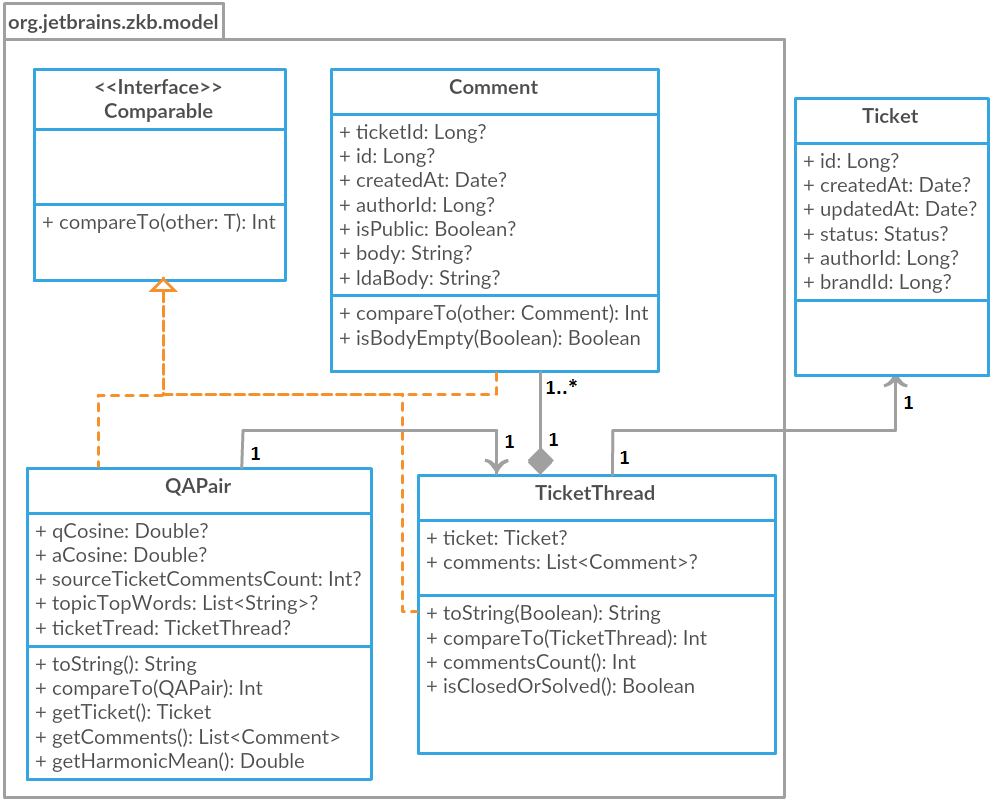
\includegraphics[width=11cm]{fig/model.png}}
    \caption{Диаграмма классов пакета org.jetbrains.zkb.model}
    \label{fig:umodel}
\end{figure}

Каждый из приведенных на рисунке~\ref{fig:umodel} классов поддерживает сериализацию в формат JSON. Поддержка сериализации объектов необходима для организации взаимодеййствия с Zendesk и MongoDB. Для этого использовалась библиотека Jackson\footnote{https://github.com/FasterXML/jackson} с добавлением к классам специальных аннотаций. В листинге~\ref{listings:comment} приведен пример класса \textit{Comment} c соответсвующими аннотациями.

\lstinputlisting[
  label={listings:comment},
  caption={Пример использования билиотеки Jackson},
  style={java}
]
{code/Comment.kt}

%%%%%%%%%%%%%%%%%%%%%%%%%%%%%%%%%%%%%%%%%%%%%%%%%%%%%%%%%%%%%%%%%%%%%%%%%%%%%%%%
\section{Взаимодействие с базой данных}
%%%%%%%%%%%%%%%%%%%%%%%%%%%%%%%%%%%%%%%%%%%%%%%%%%%%%%%%%%%%%%%%%%%%%%%%%%%%%%%%

Логика взаимодействия базой данных инкапсулирована в классах \textit{DBReader} и \textit{DBWriter}, которые располагаются в пакете \textbf{org.jetbrains.zkb.db}. Диаграмма классов данного пакета приведена на рисунке~\ref{fig:dbdmodel}.

\begin{figure}[tph!]
\centerline{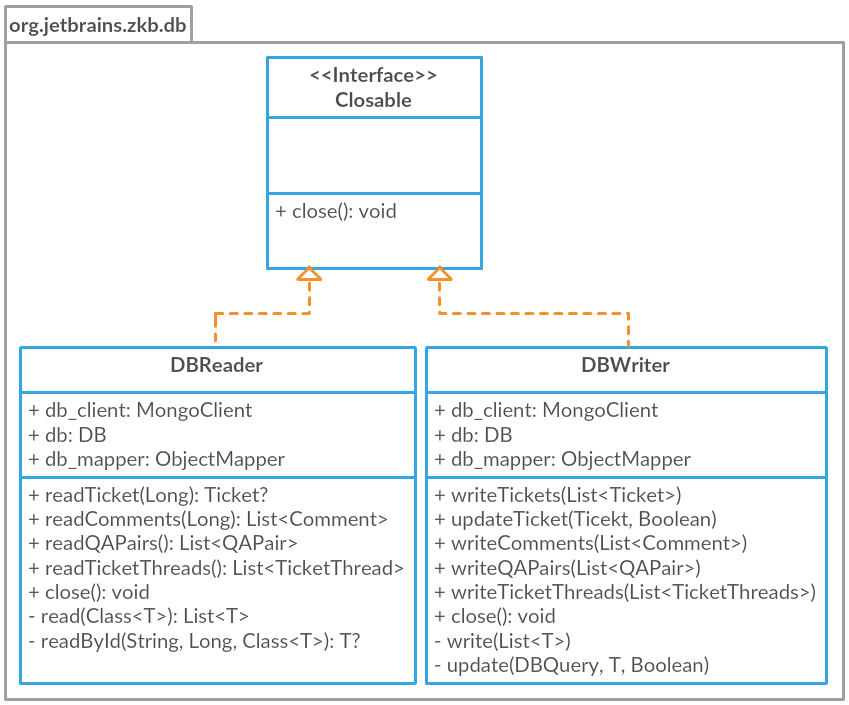
\includegraphics[width=9cm]{fig/dbmodel.png}}
    \caption{Диаграмма классов пакета org.jetbrains.zkb.db}
    \label{fig:dbdmodel}
\end{figure}

\nomenclature{BSON}{Binary JavaScript Object Notation}

MongoDB для хранения данных использует формат BSON. Класс \textit{DBReader} реализует логику трансформации объектов в JSON формат, который затем преобразуется в BSON и сохраняется в базу данных. Класс \textit{DBWriter} позволяет читать данные из базы данных, преобразуя их из BSON формата к объектам Kotlin.

%%%%%%%%%%%%%%%%%%%%%%%%%%%%%%%%%%%%%%%%%%%%%%%%%%%%%%%%%%%%%%%%%%%%%%%%%%%%%%%%
\section{Реализация предобработки данных}
%%%%%%%%%%%%%%%%%%%%%%%%%%%%%%%%%%%%%%%%%%%%%%%%%%%%%%%%%%%%%%%%%%%%%%%%%%%%%%%%
\subsection{Фильтрация данных}
\subsection{Эвристики предобработки}
%%%%%%%%%%%%%%%%%%%%%%%%%%%%%%%%%%%%%%%%%%%%%%%%%%%%%%%%%%%%%%%%%%%%%%%%%%%%%%%%
\section{Построение тематической модели}
%%%%%%%%%%%%%%%%%%%%%%%%%%%%%%%%%%%%%%%%%%%%%%%%%%%%%%%%%%%%%%%%%%%%%%%%%%%%%%%%
\subsection{Выбор реализации LDA}
\label{sec:lda_choose}
%%%%%%%%%%%%%%%%%%%%%%%%%%%%%%%%%%%%%%%%%%%%%%%%%%%%%%%%%%%%%%%%%%%%%%%%%%%%%%%%
\section{Поиск вопросно-ответных пар}
%%%%%%%%%%%%%%%%%%%%%%%%%%%%%%%%%%%%%%%%%%%%%%%%%%%%%%%%%%%%%%%%%%%%%%%%%%%%%%%%

%%%%%%%%%%%%%%%%%%%%%%%%%%%%%%%%%%%%%%%%%%%%%%%%%%%%%%%%%%%%%%%%%%%%%%%%%%%%%%%%
\section{Резюме}
%%%%%%%%%%%%%%%%%%%%%%%%%%%%%%%%%%%%%%%%%%%%%%%%%%%%%%%%%%%%%%%%%%%%%%%%%%%%%%%%

\blindtext
